\chapter{Infraestrutura atual da Empresa}
\label{cap:infraempresa}

Este capítulo apresentará a infraestrutura de \ac{TI} da empresa que será objetivo de estudo neste trabalho. Esta é uma empresa que fornece 
serviços de hospedagens e também está associada a um provedor de Internet\footnote[1]{É importante salientar que esse provedor utiliza a maior 
parte dos serviços da empresa.}. A empresa possui grande parte de seus clientes localizados na serra do Rio Grande do Sul, sendo que, atualmente, 
esta empresa possui aproximadamente 9000 clientes. A sede da empresa está localizada na cidade de Garibaldi. Além disso, a empresa possui quatro 
filiais no estado, atendendo aproximadamente 30 cidades.

A empresa oferece serviços pela Internet, sendo eles: hospedagens de sites, banco de dados, \textit{e-mail}, sistemas de gestão, 
\textit{e-mail marketing}, \textit{backup}, máquinas virtuais, autenticação via \ac{ADSL} e rádio \textit{online}. Além disso, o provedor 
associado fornece aos seus clientes acesso à Internet via rádio e acesso à Internet por meio de fibra óptica. 
A maioria dos serviços são fornecidos por meio de \textit{softwares} de código aberto.

Atualmente, a empresa possui redundância de refrigeração e de energia, como pode ser observado na Figura \ref{fig:insteletrica}. 
A redundância de refrigeração é composta por dois ares-condicionados (\textit{Ar 1 (Inverter)} e \textit{Ar 2} na Figura \ref{fig:insteletrica}). 

\begin{figure}[h!]
 \centering
 \fcolorbox{black}{white}{
  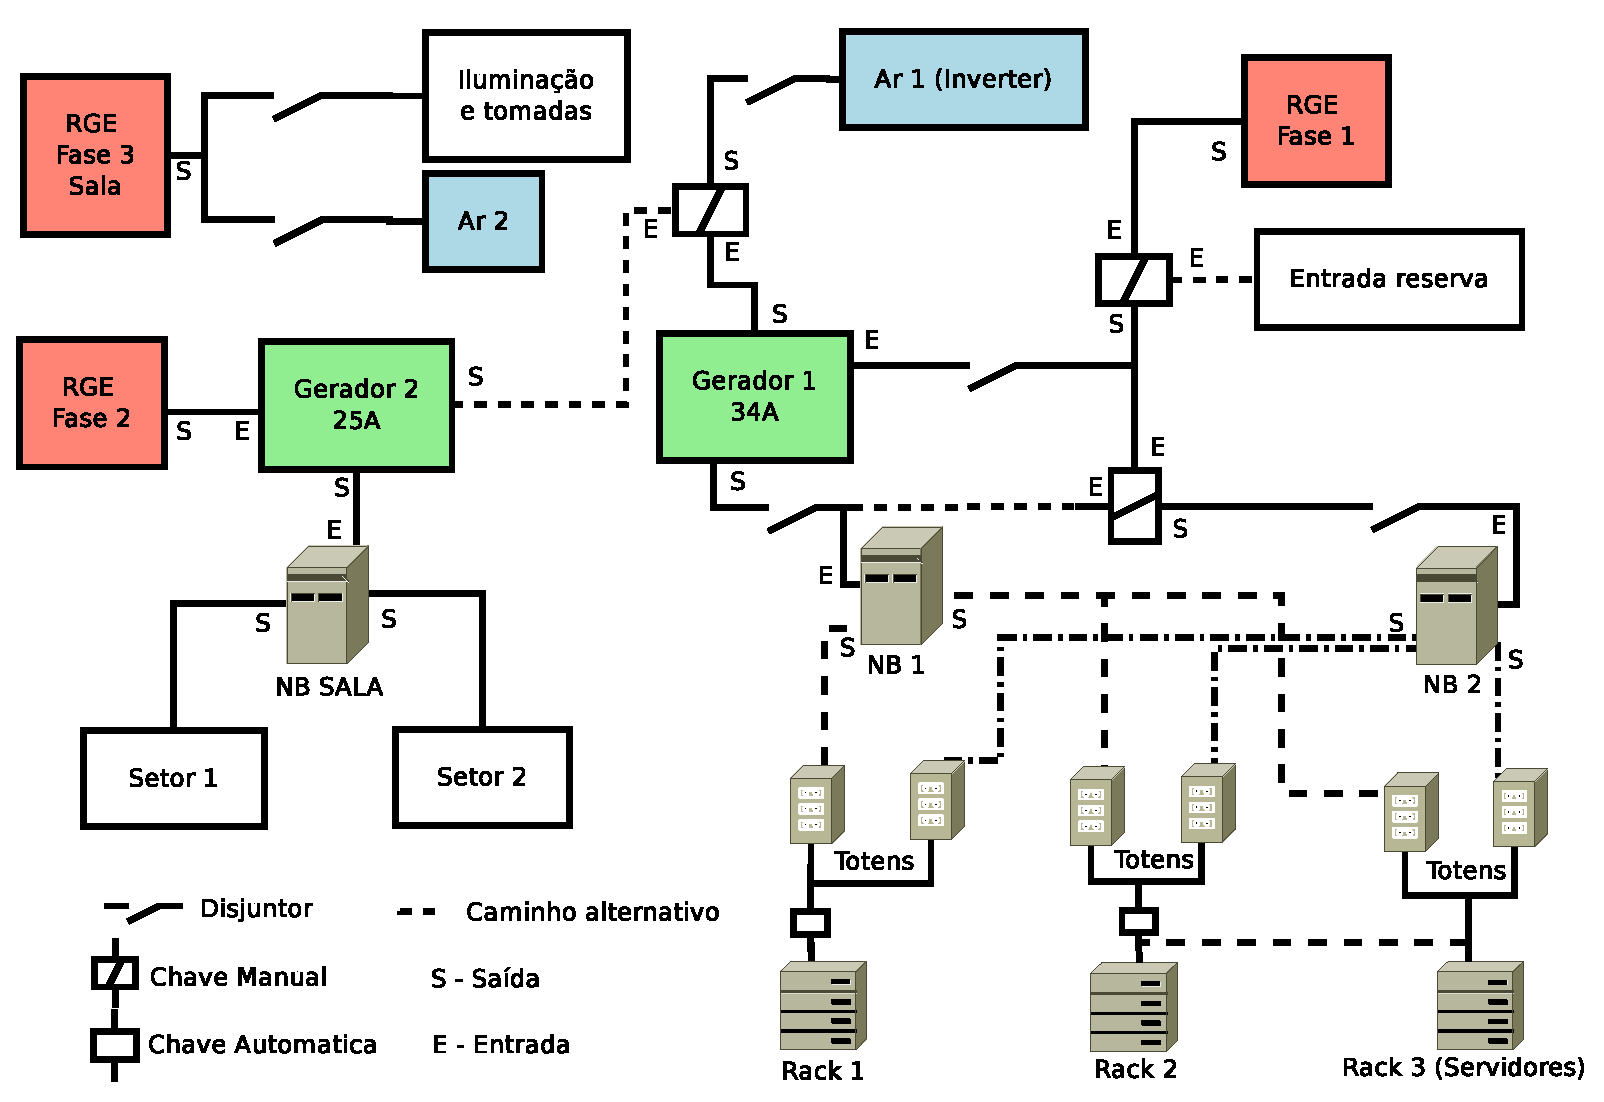
\includegraphics[width=340px]{img/insteletrica.eps}
 }
 \caption{Diagrama de instalação elétrica.}
 \label{fig:insteletrica}
\end{figure}

A redundância de energia é feita através de três \textit{nobreaks}, sendo que dois deles (identificados como \textit{NB 1} e \textit{NB 2} na 
Figura \ref{fig:insteletrica}) são utilizados para a alimentação dos servidores e outros equipamentos, como por exemplo, roteadores. Assim, se um 
\textit{nobreak} falhar o outro assume a alimentação de todos os equipamentos. O terceiro \textit{nobreak} (identificado como \textit{NB Sala} 
na Figura \ref{fig:insteletrica}) é utilizado para alimentar os computadores dos funcionários de dois setores da empresa. Conectado aos 
\textit{nobreaks} estão seis \textit{totens}\footnote[1]{\textit{Totens} são torres que possuem tomadas para plugar os equipamentos} de energia, 
sendo que nestes \textit{totens} são ligados os equipamentos e os servidores que estão localizados nos \textit{racks}. Além disso, existe a 
entrada de energia, com três fases (destacadas na cor vermelho), e dois geradores (destacados na cor verde) que suprem a necessidade de consumo 
de energia elétrica do ambiente.

Nas próximas seções será feita uma descrição da estrutura da empresa. Na Seção \ref{section:fisico} serão descritos os servidores físicos, com 
suas estruturas e configurações. Na Seção \ref{section:servsemvirt} serão descritos os servidores que não utilizam virtualização, ou seja, 
os servidores que possuem os serviços instalados diretamente sobre o sistema operacional. Na Seção \ref{section:servvirt} será descrito a 
estrutura dos servidores que utilizam de virtualização e todos os serviços fornecidos por esses servidores.

\section{Instalação física}
\label{section:fisico}

A estrutura atual da empresa é composta por quatorze servidores físicos. A configuração desses servidores pode ser observada na 
Tabela \ref{tab:servfisicos}, onde tem-se o nome do servidor, o modelo, a configuração dos processadores, quantidade de memória
\ac{RAM}, número de discos rígidos e a capacidade unitária de cada disco.

\begin{table}[h!]
\caption{Configuração dos servidores físicos.}
\label{tab:servfisicos}
\begin{center}
\def\arraystretch{1}
\setlength{\tabcolsep}{0.15cm}
\begin{tabular}{|l|l|p{5.1cm}|l|p{2.1cm}|}\hline
\textbf{Servidor} & \textbf{Modelo} & \textbf{Processador} & \textbf{Memória \ac{RAM}} & \textbf{Disco} \\\hline
Bello & & 1 x Intel Core 2 Duo E6750 2.66 GHz & 2 GB DDR2 & 5,5 TB SATA\\\hline
Cacti & Dell PowerEdge 2950 & 2 x Intel Xeon E5310 1.60 GHz & 12 GB DDR2 & 2 x 73 GB SAS\\\hline
Dati & Dell PowerEdge 1850 & 2 x Intel Xeon 3.20 GHz & 4 GB DDR2 & 2 x 146 GB SCSI\\\hline
Monit & & 1 x Intel Core 2 Quad Q9550 2.83 GHz & 4 GB DDR2 & 120 GB SSD\\\hline
Nino & & 1 x Intel Core 2 Duo E4500 2.20 GHz & 4 GB DDR2 & 500 GB SATA\\\hline
Sfrunhon & & 1 x Intel Xeon X3330 2.66 GHz & 8 GB DDR2 & 750 GB SATA\\\hline
Vigilante & & 1 x Intel Pentium Dual E2180 2.00 GHz & 4 GB DDR2 & 2,5 TB SATA\\\hline
Brina & Dell PowerEdge 2950 & 2 x Intel Xeon E5410 2.33 GHz & 24 GB DDR2 & 6 x 300 GB SAS\\\hline
Fulmine & IBM System x3650 M4 & 1 x Intel Xeon E5-2650 2.00 GHz & 32 GB DDR3 & 6 x 2 TB SATA\\\hline
Piova & Dell PowerEdge R410 & 2 x Intel Xeon E5530 2.40 GHz & 32 GB DDR3 & 4 x 500G SATA\\\hline
Raggio & HP ProLiant DL360 G7 & 2 x  Intel Xeon E5630 2.53 GHz & 32 GB DDR3 & 4 x 300 GB SAS\\\hline
Tempesta & Dell PowerEdge R620 & 2 x Intel Xeon E5-2620 2.00 GHz & 32 GB DDR3 & 5 x 1 TB SATA 3 x 1,2 TB SAS\\\hline
Tuono & HP ProLiant DL380 G7 & 2 x Intel Xeon E5649 2.53 GHz & 32 GB DDR3 & 6 x 300 GB SAS 2 x 146 GB SAS\\\hline
Venti & Dell PowerEdge R210 II & 1 x Intel Xeon E3-1220 3.10 GHz & 16 GB DDR3 & 2 x 3 TB SATA\\\hline
\end{tabular}
\end{center}
\end{table}

Todos os servidores estão ligados ao \textit{switch}, que provê acesso à Internet através de um roteador. Para os servidores mais importantes 
são utilizados dois cabos de rede que estão ligados a um \textit{switch} \textit{gigabit}, assim possibilitando a configuração de um 
\textit{link aggregation}, que permite configurar mais de uma interface de rede física em uma interface agregada. Através deste 
\textit{link aggregation} pode-se dobrar a capacidade de tráfego de dados e obter redundância de interfaces. 
O diagrama da Figura \ref{fig:servfisicos} demonstra uma visão geral da estrutura dos servidores da empresa. 

\begin{figure}[h!]
 \centering
 \fcolorbox{black}{white}{
  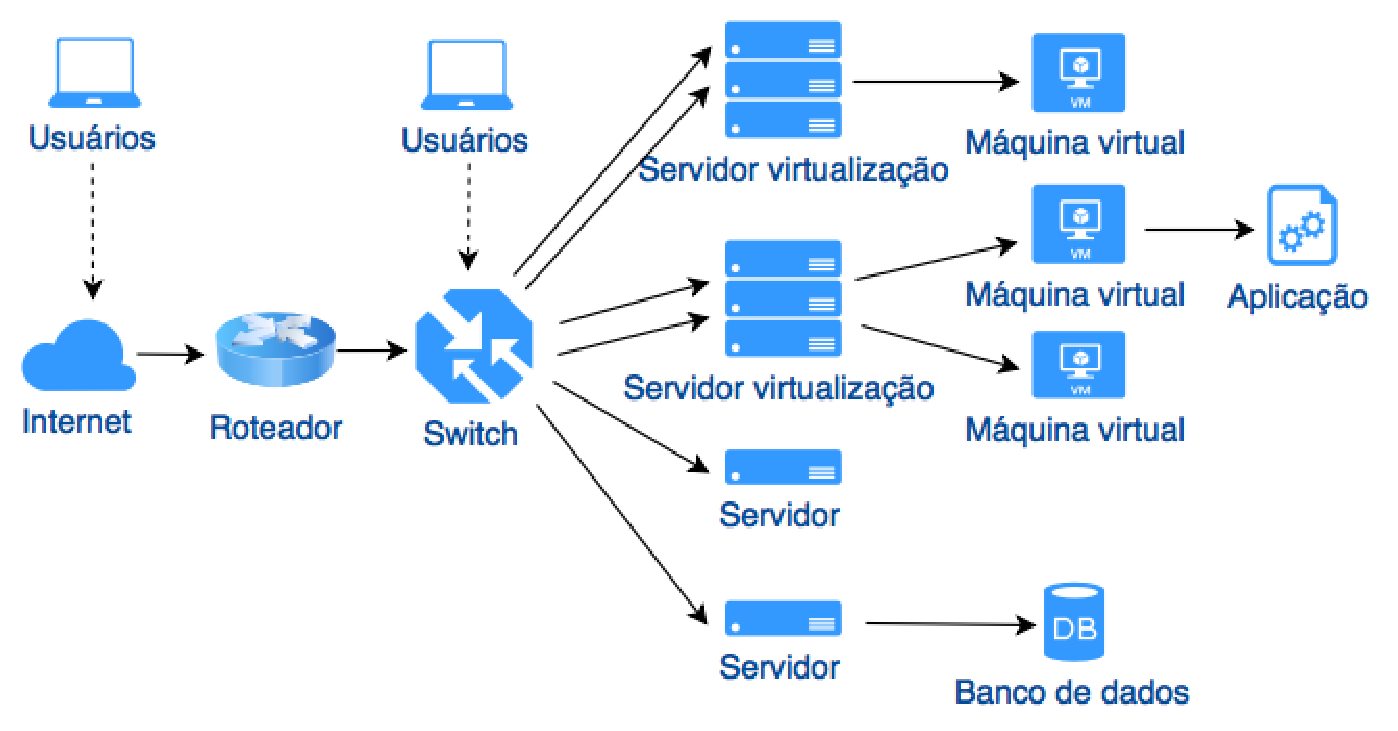
\includegraphics[width=380px]{img/servfisicos.eps}
 }
 \caption{Modelo de estrutura física.}
 \label{fig:servfisicos}
\end{figure}

A Figura \ref{fig:servrack} apresenta uma foto, com o \textit{rack} e todos os servidores, inclusive o \textit{switch}.

\begin{figure}[h!]
 \centering
 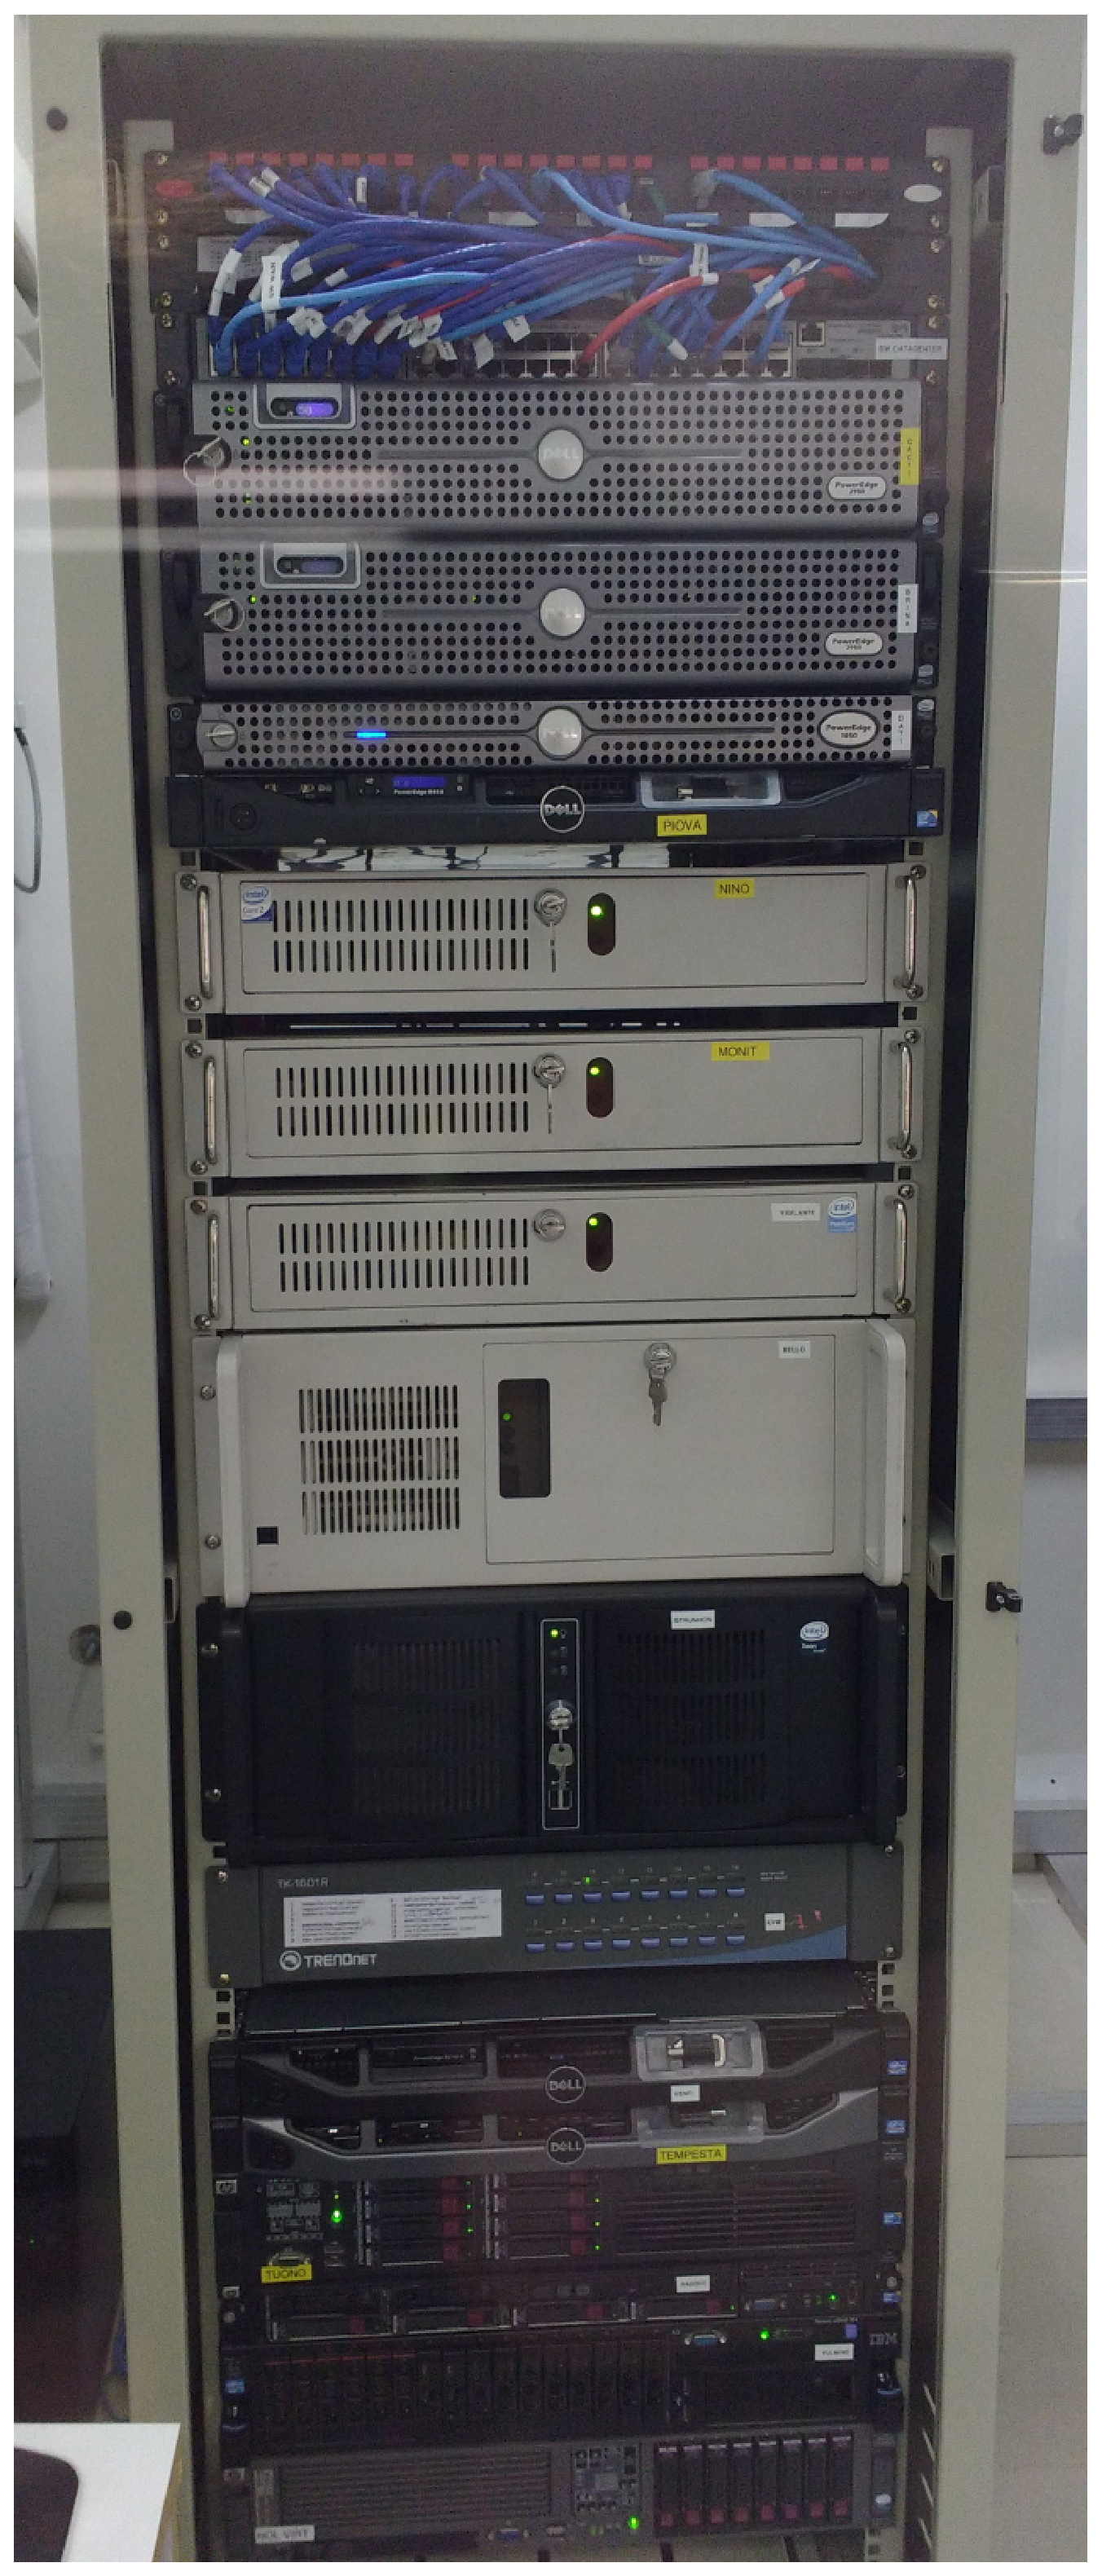
\includegraphics[width=120px]{img/servrack.eps}
 \caption{Imagem do \textit{rack} e dos servidores.}
 \label{fig:servrack}
\end{figure}

\section{Servidores sem virtualização}
\label{section:servsemvirt}

Atualmente tem-se sete servidores que possuem os serviços executando sobre o sistema operacional nativo, ou seja, sem virtualização. 
Esses são os sete primeiros servidores da Tabela \ref{tab:servfisicos}, e estão descritos abaixo:
\begin{itemize}
 \item \textit{Bello}: esse servidor possui o sistema operacional \textit{Ubuntu 14.04 \ac{LTS}} \cite{ubuntu}. Sua função é armazenar todos os 
 dados de \textit{backup} da empresa. Para isso ele possui instalado a ferramenta \textit{Bacula Storage 5.2.6} \cite{bacula}. De fato, esse só
 armazena os dados do \textit{backup}, ou seja, esse servidor não é responsável pela execução do \textit{backup}. A ferramenta que faz a execução e
 a gerência do \textit{backup} é o \textit{Bacula Director}, que encontra-se instalado no servidor \textit{Quebei} o qual será detalhado na 
 Seção \ref{section:serv_venti};
 
 \item \textit{Cacti}: um dos servidores de monitoramento da rede do provedor. Esse utiliza a distribuição \textit{CentOS 6.6} \cite{centos} e 
 executa a aplicação \textit{Cacti 0.8.8b} \cite{cacti}, que é uma ferramenta de código aberto desenvolvida para monitorar equipamentos de rede 
 que suportem o protocolo \ac{SNMP} \cite{kurose2006}. Essa ferramenta monitora a maior parte da rede 
 \textit{core}\footnote[1]{A rede \textit{core} é a rede de transporte do provedor, onde trafega os principais \textit{link} de acesso à Internet.} 
 e da rede \textit{backbone}\footnote[2]{A rede \textit{backbone} é a rede de transporte entre os pontos de atendimento a clientes.}, 
 tanto dos clientes de Internet via rádio, como de fibra óptica;
 
 \item \textit{Dati}: é o servidor de banco de dados principal, sendo que esse possui o sistema operacional \textit{Ubuntu 14.04 \ac{LTS}} 
 \cite{ubuntu}. O serviço que executa sobre esse servidor é um sistema gerenciador de banco de dados \textit{MySQL 5.5.49} \cite{mysql}, que 
 armazena os dados das aplicações \textit{ZoneMinder} \cite{zoneminder}, \textit{Icewarp Server} \cite{icewarp} e \textit{Ejabberd} \cite{ejabberd}. 
 Essas aplicações estão executando nos servidores \textit{Vigilante} (servidor de câmeras), \textit{Merak} (servidor de \textit{e-mail}) e 
 \textit{Parla} (servidor de mensagens instantâneas), respectivamente. Esses servidores serão detalhados na Seção \ref{section:servvirt};
 
 \item \textit{Monit}: esse servidor faz o monitoramento dos demais servidores. Ele possui o sistema operacional \textit{Ubuntu 12.04 \ac{LTS}} 
 \cite{ubuntu}, e executa as aplicações \textit{Nagios 3.2.3} \cite{nagios} e \textit{Munin 1.4.6} \cite{munin}, ambos \textit{softwares} livres. 
 O \textit{Nagios} é responsável por monitorar o \textit{hardware} e os serviços que estão executando em cada servidor. Já o \textit{Munin} é 
 responsável por gerar gráficos de monitoramento. Com o \textit{Munin} pode-se criar, por exemplo, gráficos com a utilização do processador, 
 de memória \ac{RAM}, do disco rígido, da temperatura e da velocidade dos \textit{fans}\footnote[3]{Os \textit{fans} são exaustores, ou seja, 
 ventiladores que empurram o ar quente para fora de um recipiente ou ambiente \cite{ats2012}.};
 
 \item \textit{Nino}: esse é o servidor utilizado pelo setor de desenvolvimento de \textit{software}. Suas aplicações executam sobre o sistema 
 operacional \textit{Ubuntu 14.04 \ac{LTS}} \cite{ubuntu}, sendo que os serviços fornecidos pelo servidor são: um servidor \textit{Web} 
 \textit{Apache 2.4.7} \cite{apache}; \textit{\ac{PHP} 5.5.9} \cite{php}; sistema gerenciador de banco de dados \textit{MySQL 5.5.49} \cite{mysql} 
 e \textit{PostgreSQL 9.3.13} \cite{postgres}; compartilhamento de arquivos \textit{Samba 4.3.9} \cite{samba}; controle de versões de 
 \textit{software} \textit{\ac{SVN} 1.8.8} \cite{svn}; gerenciador de \textit{bugs} \textit{Trac 1.0.1} \cite{trac}; e o gerenciador de 
 mensagens instantâneas para ambiente de testes \textit{Ejabberd 2.1.11} \cite{ejabberd};
 
 \item \textit{Sfrunhon}: é um servidor de monitoramento da rede do provedor. Esse utiliza a distribuição \textit{CentOS 6.3} \cite{centos} e 
 executa a aplicação \textit{Cacti 0.8.8a} \cite{cacti}. Esse servidor monitora o tráfego de dados dos clientes do provedor, tanto de Internet 
 via rádio, como de fibra óptica;
 
 \item \textit{Vigilante}: esse servidor é responsável por capturar e armazenar o \textit{streaming} de vídeo das câmeras de segurança do provedor. 
 Esse possui o sistema operacional \textit{Ubuntu 14.04 \ac{LTS}} \cite{ubuntu} e executa a aplicação \textit{ZoneMinder 1.29} \cite{zoneminder}, 
 que é a aplicação responsável pela captura e armazenamento das imagens das câmeras do provedor.
\end{itemize}

\section{Servidores com virtualização}
\label{section:servvirt}

Os servidores de virtualização possuem suas respectivas \ac{VM}s, sendo que, para a criação dessas \ac{VM}s utiliza-se o hipervisor \ac{KVM} 
\cite{kvm} e a ferramenta \textit{QEmu}, que são projetos de \textit{software} livre. Procurou-se manter um ambiente homogêneo com o objetivo de 
facilitar a manutenção, para isso utilizou-se o mesmo hipervisor e o mesmo sistema operacional hospedeiro. Esse sistema operacional é o sistema 
de código aberto \textit{Ubuntu 14.04 \ac{LTS}} \cite{ubuntu}. Além disso, esses servidores possuem redundância de \textit{hardware}, com fonte 
de alimentação duplicada e discos rígidos configurados através de \ac{RAID} \cite{raid}. Em servidores com mais de dois discos é utilizado 
\ac{RAID} 5 \cite{raid}. Já em servidores que possuem apenas dois discos é utilizado \ac{RAID} 1 (espelhamento de discos) \cite{raid}. 
O ambiente também possui redundância no cabeamento de rede, como visto anteriormente.

A empresa fornece serviços diversos, desde hospedagens de sites até \ac{DNS} recursivo para o provedor de Internet. Atualmente sete servidores 
são utilizados com virtualização (os últimos sete servidores da Tabela \ref{tab:servfisicos}), sendo que existem quarenta e seis \ac{VM}s 
distribuídas entre esses sete servidores. Nas próximas seções serão descritos esses servidores, e as respectivas máquinas virtuais que são
executadas nestes.

\subsection{Servidor Brina}
\label{section:serv_brina}

O servidor Brina possui duas \ac{VM}s, como pode ser visto na Figura \ref{fig:servidor_brina}, sendo que os serviços executados nas \ac{VM}s são:

\begin{figure}[h!]
 \centering
 \fcolorbox{black}{white}{
  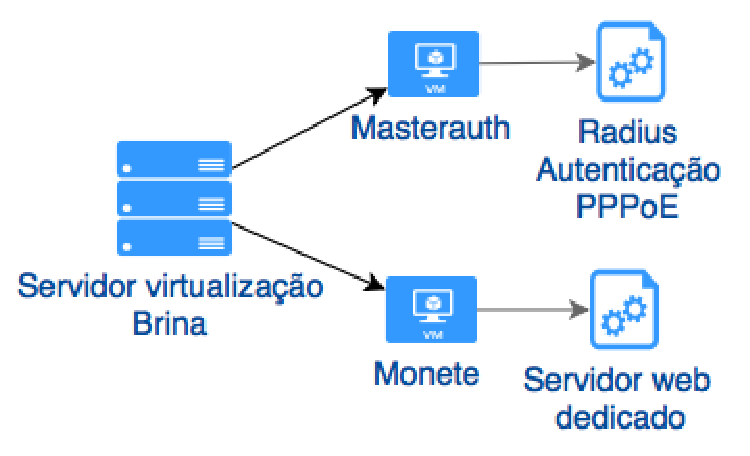
\includegraphics[width=180px]{img/servidor_brina.eps}
 }
 \caption{Servidor de virtualização Brina.}
 \label{fig:servidor_brina}
\end{figure}

\begin{itemize}
 \item \textit{Masterauth}: sua configuração é de 1 \textit{core} de \textit{2.33 GHz}, 1,5 GB de memória \ac{RAM} e 8 GB de disco. 
 O sistema operacional é o \textit{Ubuntu 14.04 \ac{LTS}} \cite{ubuntu}, sendo que esse servidor virtual fornece um serviço de autenticação 
 \ac{PPPoE} \cite{javvin2005} para uma parte dos clientes do provedor. Para a autenticação é utilizada o \textit{software} 
 \textit{Freeradius 2.1.12} \cite{freeradius};
 
 \item \textit{Monete}: sua configuração é de 1 \textit{core} de \textit{2.33 GHz}, 3 GB de memória \ac{RAM} e 50 GB de disco. 
 Esse servidor possui o sistema operacional \textit{Ubuntu 14.04 \ac{LTS}} \cite{ubuntu} e é um servidor \textit{Web} dedicado para o site do 
 provedor, ou seja, esse servidor armazena o site do provedor. Para isso ele utiliza os \textit{softwares} 
 \textit{Apache 2.4.7} \cite{apache}, \textit{\ac{PHP} 5.5.9} \cite{php} e \textit{MySQL 5.5.49} \cite{mysql}.
\end{itemize}

\subsection{Servidor Fulmine}
\label{section:serv_fulmine}

O servidor Fulmine possui dez \ac{VM}s, como pode ser visto na Figura \ref{fig:servidor_fulmine}, sendo que os serviços executados nas \ac{VM}s são:

\begin{figure}[h!]
 \centering
 \fcolorbox{black}{white}{
  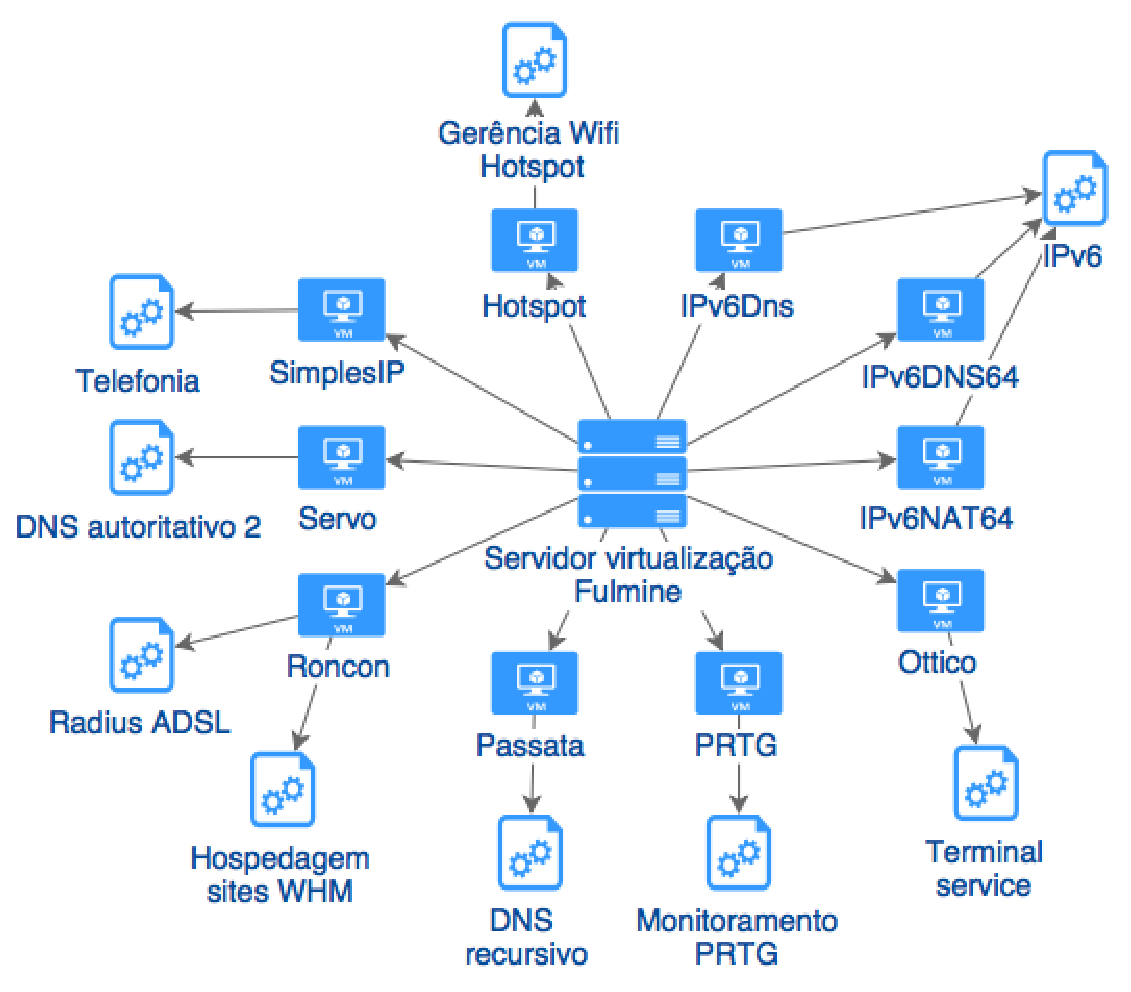
\includegraphics[width=310px]{img/servidor_fulmine.eps}
 }
 \caption{Servidor de virtualização Fulmine.}
 \label{fig:servidor_fulmine}
\end{figure}

\begin{itemize}
 \item \textit{Hotspot}: sua configuração é de 1 \textit{core} de \textit{2.0 GHz}, 1,5 GB de memória \ac{RAM} e 8 GB de disco. 
 Esse servidor virtual possui o sistema operacional \textit{Ubuntu 14.04 \ac{LTS}} \cite{ubuntu}, sendo que esse servidor faz a gerência de 
 equipamentos da \textit{Ubiquiti} que fazem \textit{hotspot}\footnote[1]{\textit{Hotspot} é um tipo de rede sem fim para computadores móveis 
 e normalmente estão presentes em locais como hotéis, aeroportos, entre outros \cite{tanenbaum2011}.}. Esses equipamentos disponibilizam a 
 tecnologia \textit{Wi-fi} para prover acesso à Internet em ambientes públicos e são utilizados pelo provedor;
 
 \item \textit{IPv6Dns}, \textit{IPv6Dns64} e \textit{IPv6Nat64}: suas configurações são de 1 \textit{core} de \textit{2.0 GHz}, 
 1 GB de memória \ac{RAM} e 8 GB de disco. O sistema operacional é o \textit{Ubuntu 14.04 \ac{LTS}} \cite{ubuntu}, sendo que essas \ac{VM}s
 fornecem o serviço de \ac{DNS} \cite{tanenbaum2011} e \ac{NAT} \cite{kurose2006} para navegação \ac{IPv6} \cite{ipv6} do provedor;
 
 \item \textit{Ottico}: esse servidor possui 2 \textit{cores} de \textit{2.0 GHz}, 4 GB de memória \ac{RAM} e 50 GB de disco. 
 O servidor possui o sistema operacional \textit{Windows 2007 Server Standard} e possui o serviço de \textit{terminal service} para suporte e 
 gerência da infraestrutura de fibra óptica do provedor;
 
 \item \ac{PRTG}: esse servidor possui 2 \textit{cores} de \textit{2.0 GHz}, 4 GB de memória \ac{RAM} e 100 GB de disco. 
 O servidor possui o sistema operacional \textit{Windows 2008 Server R2} e sua função é monitorar o tráfego de rede dos equipamentos da 
 rede \textit{core} do provedor;
 
 \item \textit{Passata}: esse servidor possui 2 \textit{cores} de \textit{2.0 GHz}, 3 GB de memória \ac{RAM} e 20 GB de disco. 
 O servidor possui o sistema operacional \textit{Ubuntu 14.04 \ac{LTS}} \cite{ubuntu} e fornece o serviço de \ac{DNS} recursivo, através do 
 \textit{software} \textit{Bind 9.9.5} \cite{bind}. Esse é o servidor primário de \ac{DNS}, sendo o mais importante para navegação dos clientes 
 do provedor;
 
 \item \textit{Roncon}: esse servidor possui 4 \textit{cores} de \textit{2.0 GHz}, 6 GB de memória \ac{RAM} e 400 GB de disco. 
 Ele possui o sistema operacional \textit{Red Hat 5.11} \cite{redhat} e provê hospedagem de sites \textit{Web} desenvolvidos com a linguagem 
 \ac{PHP}. Nele está instalado o \textit{software} \ac{WHM} \cite{whm}, que faz a gerência dos serviços de hospedagens desses sites e de banco de 
 dados. Além disso, encontra-se disponível a ferramenta \textit{cPanel}, que faz parte do \ac{WHM} e fornece acesso aos desenvolvedores de
 sites. Para fornecer a hospedagem desses sites os seguintes \textit{softwares} estão instalados: \textit{Apache 2.2.26} \cite{apache}, 
 \textit{\ac{PHP} 5.3.27} \cite{php}, \textit{MySQL 5.1.73} \cite{mysql} e \textit{PostgreSQL 8.4.20} \cite{postgres}.
 Além da hospedagem, esse servidor fornece o serviço de autenticação \ac{ADSL} \cite{tanenbaum2011} de terceiros utilizando o \textit{software} 
 \textit{Freeradius 1.1.3} \cite{freeradius};
 
 \item \textit{Servo}: sua configuração é de 1 \textit{core} de \textit{2.0 GHz}, 2 GB de memória \ac{RAM} e 30 GB de disco. 
 Esse servidor possui o sistema operacional \textit{CentOS 6.8} \cite{centos}, sendo que este servidor virtual fornece, através do \textit{software} 
 \textit{Bind 9.8.2} \cite{bind}, o serviço de \ac{DNS} autoritativo. Esse é o servidor de \ac{DNS} secundário dos domínios hospedados pela empresa;
 
 \item \textit{SimplesIP}: esse servidor possui 2 \textit{cores} de \textit{2.0 GHz}, 3 GB de memória \ac{RAM} e 80 GB de disco. 
 O servidor possui o sistema operacional \textit{CentOS 6.6} \cite{centos} e é o servidor de telefonia sobre \ac{IP} do provedor. Esse utiliza 
 como base o \textit{software} \textit{Asterisk 1.8.32} \cite{asterisk}.
\end{itemize}

\subsection{Servidor Piova}
\label{section:serv_piova}

O servidor Piova possui nove \ac{VM}s, como pode ser visto na Figura \ref{fig:servidor_piova}, sendo que os serviços executados nas \ac{VM}s são:

\begin{figure}[h!]
 \centering
 \fcolorbox{black}{white}{
  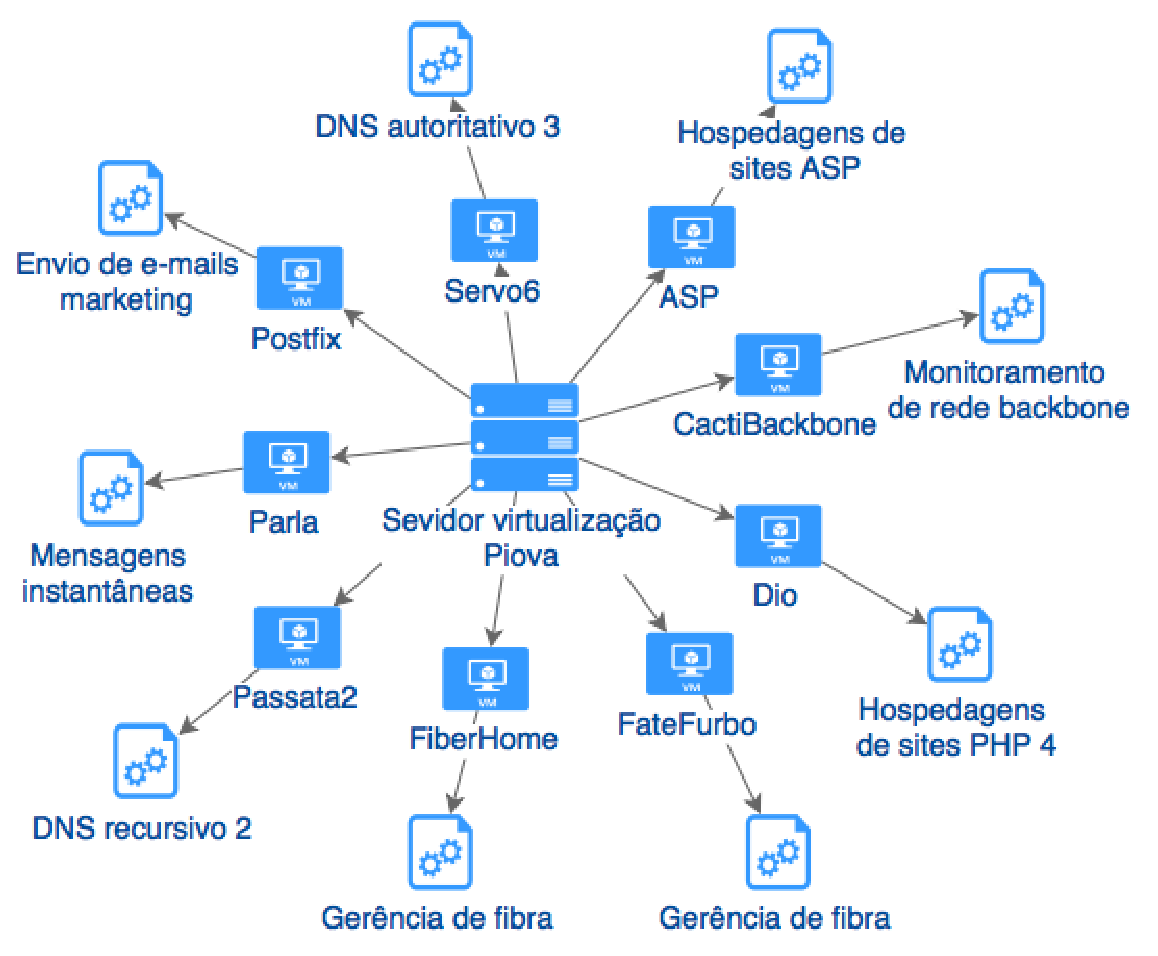
\includegraphics[width=320px]{img/servidor_piova.eps}
 }
 \caption{Servidor de virtualização Piova.}
 \label{fig:servidor_piova}
\end{figure}

\begin{itemize}
 \item \textit{ASP}: esse servidor possui 1 \textit{core} de \textit{2.40 GHz}, 1 GB de memória \ac{RAM} e 50 GB de disco. 
 O servidor possui o sistema operacional \textit{Windows 2008 Server R2} e provê acesso a sites \textit{Web} desenvolvidos com a linguagem 
 \ac{ASP} \cite{asp}, através do \textit{software} \textit{\ac{IIS} 7.5} \cite{iis}. Destaca-se que esse servidor hospeda um número baixo de sites.
 De fato, esse armazena somente 10 sites;
 
 \item \textit{CactiBackbone}: esse servidor possui 1 \textit{core} de \textit{2.40 GHz}, 1 GB de memória \ac{RAM} e 20 GB de disco. 
 Ele é um servidor de monitoramento da rede do provedor. Esse utiliza a distribuição \textit{CentOS 6.3} \cite{centos} e executa a aplicação 
 \textit{Cacti 0.8.8a} \cite{cacti}. Essa aplicação monitora atualmente uma parte da rede \textit{backbone} do provedor;
 
 \item \textit{Dio}: esse servidor possui 1 \textit{core} de \textit{2.40 GHz}, 1 GB de memória \ac{RAM} e 17,8 GB de disco. 
 O servidor possui o sistema operacional \textit{Ubuntu 6.06 \ac{LTS}} \cite{ubuntu} e fornece serviço de hospedagens de sites desenvolvidos com 
 a linguagem \ac{PHP} versão 4.4.2. Esses sites são mantidos em um servidor separado devido a incompatibilidade com a versão 5. Esse servidor 
 armazena somente 10 sites;
 
 \item \textit{FateFurbo}: sua configuração é de 2 \textit{cores} de \textit{2.40 GHz}, 4 GB de memória \ac{RAM} e 80 GB de disco. 
 O sistema operacional é o \textit{Ubuntu 14.04 \ac{LTS}} \cite{ubuntu}. Esse servidor possui um \textit{software} proprietário da empresa 
 \textit{Padtec}, que faz a gerência de uma parte da rede de fibra óptica do provedor;
 
 \item \textit{FiberHome}: sua configuração é de 2 \textit{cores} de \textit{2.40 GHz}, 2 GB de memória \ac{RAM} e 60 GB de disco. 
 Esse servidor possui o sistema operacional \textit{Windows XP} e possui o \textit{software} \textit{ANM 2000} instalado. Esse \textit{software} 
 é utilizado para a gerência da fibra óptica do provedor;
 
 \item \textit{Parla}: sua configuração é de 1 \textit{core} de \textit{2.40 GHz}, 1 GB de memória \ac{RAM} e 8 GB de disco. 
 Ele possui o sistema operacional \textit{Ubuntu 14.04 \ac{LTS}} \cite{ubuntu} e provê um serviço de mensagens instantâneas, baseado no protocolo 
 \ac{XMPP} \cite{xmpp}. Esse serviço é utilizado para comunicação entre funcionários da empresa e do provedor, e também entre os clientes e 
 os funcionários. O \textit{software} utilizado é o \textit{Ejabberd 2.1.11} \cite{ejabberd}, que também é um \textit{software} de código aberto;

 \item \textit{Passata2}: esse servidor possui 1 \textit{core} de \textit{2.40 GHz}, 2 GB de memória \ac{RAM} e 20 GB de disco. 
 Esse servidor possui o sistema operacional \textit{Ubuntu 14.04 \ac{LTS}} \cite{ubuntu} e fornece o serviço de \ac{DNS} recursivo, através do 
 \textit{software} \textit{Bind 9.9.5} \cite{bind}. Esse é o servidor secundário de \ac{DNS} do provedor;
 
 \item \textit{Postfix}: sua configuração é de 1 \textit{core} de \textit{2.40 GHz}, 768 MB de memória \ac{RAM} e 50 GB de disco. 
 Esse servidor possui o sistema operacional \textit{Ubuntu 14.04 \ac{LTS}} \cite{ubuntu} e é responsável pelo envio de \textit{e-mails}, 
 através do \textit{software} \textit{Postfix 2.11} \cite{postfix}. Os \textit{e-mails} enviados por esse servidor são gerados por uma 
 ferramenta de \textit{e-mail marketing}, que foi desenvolvida pela empresa. Ou seja, esse servidor faz o envio de \textit{e-mails} em massa 
 para divulgação de informações ou produtos;
 
 \item \textit{Servo6}: sua configuração é de 1 \textit{core} de \textit{2.40 GHz}, 1,5 GB de memória \ac{RAM} e 30 GB de disco. 
 Esse servidor possui o sistema operacional \textit{CentOS 6.8} e fornece, através do \textit{software} \textit{Bind 9.8.2} \cite{bind}, o 
 serviço de \ac{DNS} autoritativo. Esse é o servidor de \ac{DNS} terciário dos domínios hospedados pela empresa.
\end{itemize}

\subsection{Servidor Raggio}
\label{section:serv_raggio}

O servidor chamado Raggio executa doze \ac{VM}s (Figura \ref{fig:servidor_raggio}), que fornecem os serviços de virtualização para algumas empresas,
sendo que as máquinas virtuais são instaladas com o sistema operacional de preferência do cliente. O acesso a essas máquinas virtuais é realizado
através de um serviço de acesso remoto, como por exemplo, o de \ac{SSH} \cite{barrett2005}.

\begin{figure}[h!]
 \centering
 \fcolorbox{black}{white}{
  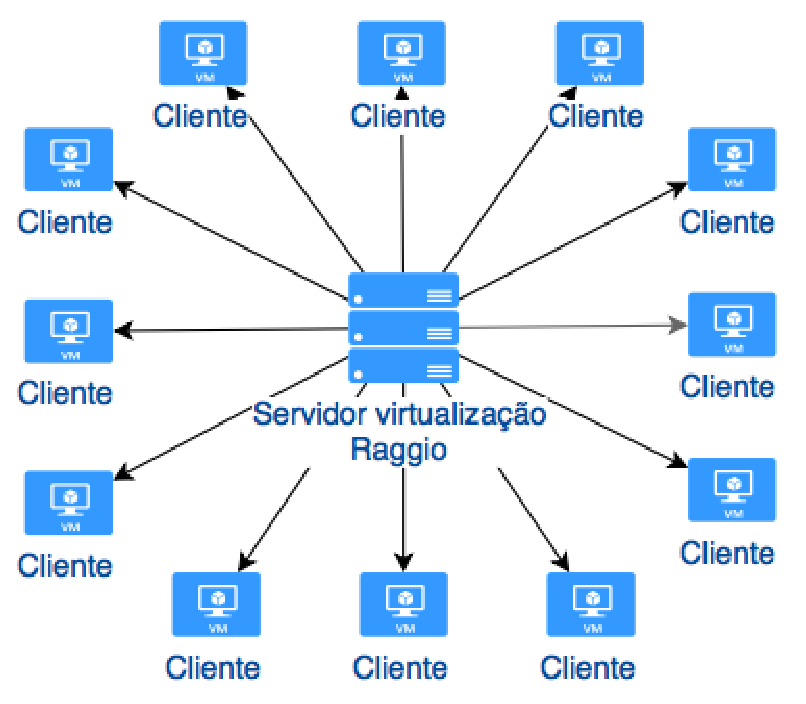
\includegraphics[width=220px]{img/servidor_raggio.eps}
 }
 \caption{Servidor de virtualização Raggio.}
 \label{fig:servidor_raggio}
\end{figure}

\subsection{Servidor Tempesta}
\label{section:serv_tempesta}

O servidor Tempesta possui quatro \ac{VM}s, como pode ser visto na Figura \ref{fig:servidor_tempesta}, sendo que os serviços executados nas 
\ac{VM}s são:

\begin{figure}[h!]
 \centering
 \fcolorbox{black}{white}{
  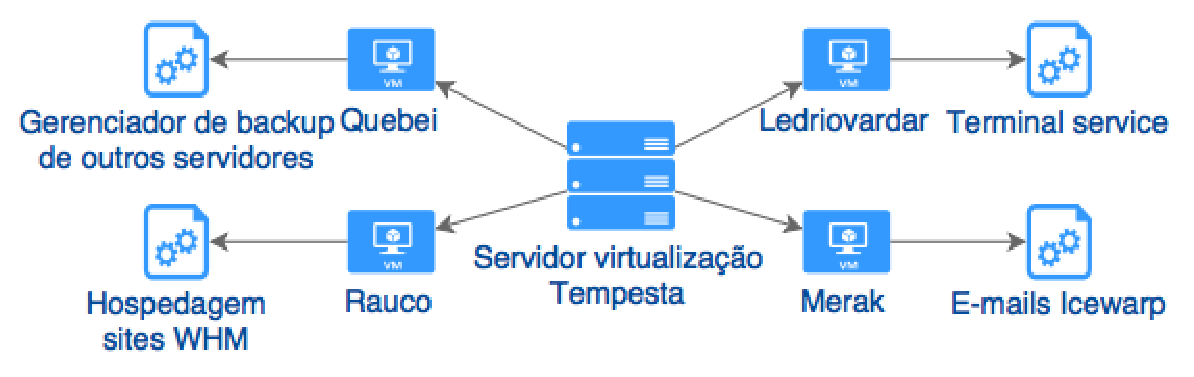
\includegraphics[width=350px]{img/servidor_tempesta.eps}
 }
 \caption{Servidor de virtualização Tempesta.}
 \label{fig:servidor_tempesta}
\end{figure}

\begin{itemize}
 \item \textit{Ledriovardar}: esse servidor possui 2 \textit{cores} de \textit{2.40 GHz}, 2 GB de memória \ac{RAM} e 80 GB de disco. 
 O servidor possui o sistema operacional \textit{Windows 2008 Server R2} e possui o serviço de \textit{terminal service} para suporte e gerência 
 da rede do provedor;
 
 \item \textit{Merak}: esse servidor fornece serviço de \textit{e-mail}. Ele possui uma configuração de 6 \textit{cores} de \textit{2.00 GHz}, 
 10 GB de memória \ac{RAM} e 1 TB de disco. O servidor possui o sistema operacional \textit{Windows 2008 Server R2} e executa o \textit{software} 
 \textit{Icewarp Server 10.4.4} \cite{icewarp}. Essa aplicação fornece os serviços de envios de: \textit{e-mails} através do protocolo 
 \ac{SMTP} \cite{kurose2006}; recebimentos de \textit{e-mails} através dos protocolos \ac{POP} \cite{kurose2006} e \ac{IMAP} \cite{kurose2006}; 
 e o serviço de \textit{Webmail} (\ac{PHP}) e Anti-spam. Destaca-se que grande parte das contas de \textit{e-mail} estão ociosas pois são oferecidas 
 juntamente com o serviço de Internet fornecida pelo provedor;
 %Possui ?? contas sendo que possui uma média de ?? usuários simultâneos...
 
 \item \textit{Quebei}: sua configuração é de 1 \textit{core} de \textit{2.00 GHz}, 3 GB de memória \ac{RAM} e 140 GB de disco. 
 Esse servidor possui o sistema operacional \textit{Ubuntu 14.04 \ac{LTS}} \cite{ubuntu} e sua função é gerenciar o \textit{backup} dos outros 
 servidores. Para isso ele utiliza a ferramenta \textit{Bacula 5.2.6} \cite{bacula} (pacote \textit{bacula-director-common 5.2.6}). Destaca-se
 que esse \textit{backup} é armazenado no servidor físico \textit{Bello}, que foi detalhado na Seção \ref{section:servsemvirt}. Além disso, 
 esse servidor possui o sistema gerenciador de banco de dados \textit{MySQL 5.5.49} \cite{mysql} instalado, que está configurado no modelo 
 \textit{master-slave}, sendo que esse servidor é o \textit{slave} e o servidor \textit{Dati} é o \textit{master};
 
 \item \textit{Rauco}: esse servidor possui 2 \textit{cores} de \textit{2.00 GHz}, 6 GB de memória \ac{RAM} e 600 GB de disco. 
 Ele possui o sistema operacional \textit{CentOS 6.8} \cite{centos}. Ou seja, esse servidor virtual fornece o mesmo serviço do servidor \textit{Roncon}, 
 que foi descrito na Seção \ref{section:serv_fulmine}. Esse servidor fornece acesso a sites \textit{Web} desenvolvidos com a linguagem \ac{PHP}. 
 Foram criados dois servidores para a hospedagem de forma a suportar um número maior de sites.
\end{itemize}

\subsection{Servidor Tuono}
\label{section:serv_tuono}

O servidor Tuono possui quatro \ac{VM}s, como pode ser visto na Figura \ref{fig:servidor_tuono}, sendo que os serviços executados nas \ac{VM}s são:

\begin{figure}[h!]
 \centering
 \fcolorbox{black}{white}{
  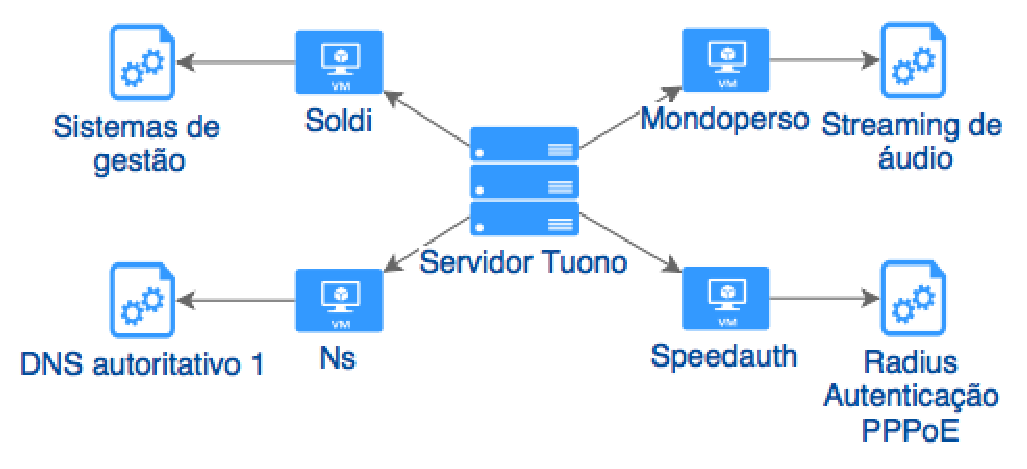
\includegraphics[width=300px]{img/servidor_tuono.eps}
 }
 \caption{Servidor de virtualização Tuono.}
 \label{fig:servidor_tuono}
\end{figure}

\begin{itemize}
 \item \textit{Mondoperso}: sua configuração é de 1 \textit{core} de \textit{2.53 GHz}, 512 MB de memória \ac{RAM} e 8 GB de disco. 
 Esse servidor possui o sistema operacional \textit{Ubuntu 14.04 \ac{LTS}} \cite{ubuntu} e fornece \textit{streaming} de áudio para uma 
 \textit{Web} rádio. Esse serviço é feito através do \textit{software} livre \textit{Icecast 2.3.3} \cite{icecast};
 
 \item \textit{Ns}: esse servidor possui 1 \textit{core} de \textit{2.53 GHz}, 2 GB de memória \ac{RAM} e 30 GB de disco. O servidor possui o sistema 
 operacional \textit{CentOS 6.8} \cite{centos} e fornece, através do \textit{software} \textit{Bind 9.9.3} \cite{bind}, o serviço de \ac{DNS} 
 autoritativo. Esse é o servidor de \ac{DNS} primário dos domínios hospedados pela empresa;

 \item \textit{Soldi}: sua configuração é 4 \textit{cores} de \textit{2.53 GHz}, 4 GB de memória \ac{RAM} e 40 GB de disco. 
 Esse servidor possui o sistema operacional \textit{Ubuntu 14.04 \ac{LTS}} \cite{ubuntu} e é um servidor \textit{Web} exclusivo para os
 \textit{softwares} de gestão que são desenvolvidos pela empresa. Os seguintes \textit{softwares} são utilizados: \textit{Apache 2.4.7} 
 \cite{apache}, \textit{\ac{PHP} 5.5.9} \cite{php} e \textit{MySQL 5.5.49} \cite{mysql};

 \item \textit{Speedauth}: sua configuração é de 2 \textit{cores} de \textit{2.53 GHz}, 1,5 GB de memória \ac{RAM} e 8 GB de disco. 
 O sistema operacional é o \textit{Ubuntu 14.04 \ac{LTS}} \cite{ubuntu}, sendo que esse servidor fornece o mesmo serviço do servidor 
 \textit{Masterauth} (Seção \ref{section:serv_brina}), que é autenticação \ac{PPPoE} dos clientes do provedor. Esse servidor é responsável pelas 
 as autenticações da maior parte dos usuários do provedor.
\end{itemize}

\subsection{Servidor Venti}
\label{section:serv_venti}

O servidor Venti possui cinco \ac{VM}s, como pode ser visto na Figura \ref{fig:servidor_venti}, sendo que os serviços executados nessas \ac{VM}s
são:

\begin{figure}[h!]
 \centering
 \fcolorbox{black}{white}{
  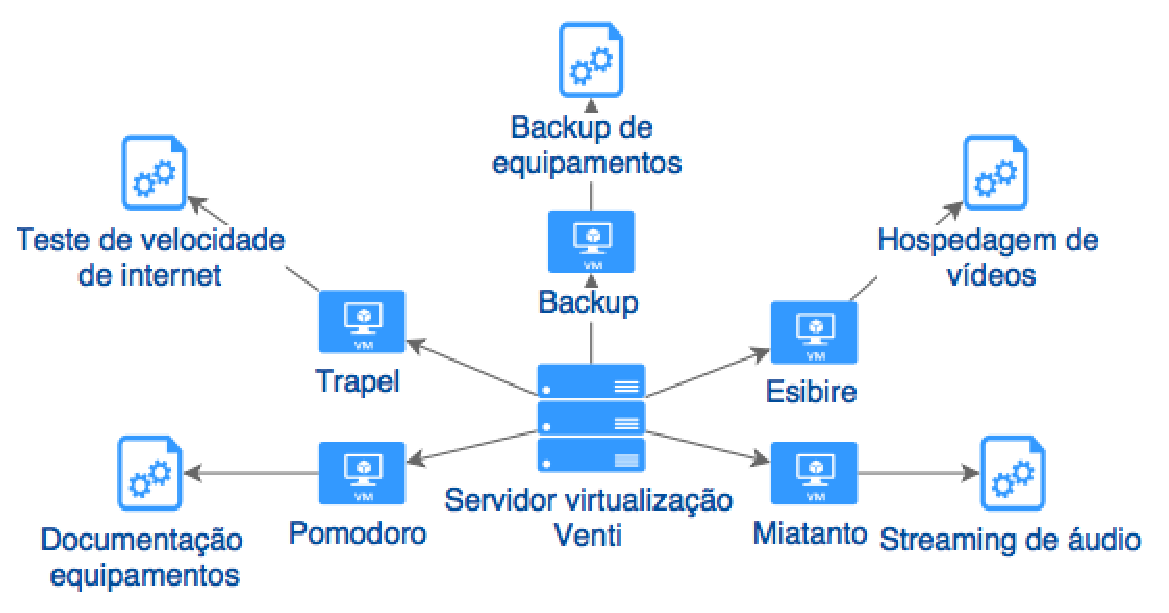
\includegraphics[width=340px]{img/servidor_venti.eps}
 }
 \caption{Servidor de virtualização Venti.}
 \label{fig:servidor_venti}
\end{figure}

\begin{itemize}
 \item \textit{Backup}: sua configuração é 1 \textit{core} de \textit{3.10 GHz}, 1 GB de memória \ac{RAM} e 15 GB de disco. 
 Esse servidor possui o sistema operacional \textit{Ubuntu 14.04 \ac{LTS}} \cite{ubuntu} e executa o serviço de \textit{backup} dos equipamentos 
 do provedor. Esse servidor utiliza \textit{scripts} que foram desenvolvidos internamente e que efetuam a cópia de dados através do protocolo 
 \ac{FTP} \cite{kurose2006};
 
 \item \textit{Esibire}: sua configuração é 1 \textit{core} de \textit{3.10 GHz}, 1 GB de memória \ac{RAM} e 50 GB de disco. 
 Esse servidor possui o sistema operacional \textit{Ubuntu 14.04 \ac{LTS}} \cite{ubuntu}, esse servidor faz a hospedagem de vídeos utilizando o 
 protocolo \ac{FTP} e faz a reprodução de \textit{streaming} utilizando um servidor \textit{Web} \textit{Apache 2.4.7};
 
 \item \textit{Miatanto}: sua configuração é 1 \textit{core} de \textit{3.10 GHz}, 1 GB de memória \ac{RAM} e 8 GB de disco. 
 Esse servidor possui o sistema operacional \textit{Ubuntu 14.04 \ac{LTS}} \cite{ubuntu} e fornece \textit{streaming} de áudio para uma \textit{Web} 
 rádio. Esse serviço é feito através do \textit{software} livre \textit{Icecast 2.3.3} \cite{icecast};
 
 \item \textit{Pomodoro}: sua configuração é 1 \textit{core} de \textit{3.10 GHz}, 2 GB de memória \ac{RAM} e 28 GB de disco. 
 Esse servidor possui o sistema operacional \textit{Ubuntu 14.04 \ac{LTS}} \cite{ubuntu} e armazena a documentação dos equipamentos do provedor. 
 Para esse armazenamento ele utiliza o \textit{software} de código aberto \textit{Sakai 2.9} \cite{sakai};
 
 \item \textit{Trapel}: sua configuração é 1 \textit{core} de \textit{3.10 GHz}, 768 MB de memória \ac{RAM} e 8 GB de disco. 
 Esse servidor possui o sistema operacional \textit{Ubuntu 14.04 \ac{LTS}} \cite{ubuntu} e fornece um serviço de teste de velocidade da conexão 
 à Internet. Ou seja, os usuários do provedor utilizam esse serviço para testar a velocidade da sua Internet. Para isso ele executa as aplicações 
 \textit{Apache 2.4.7} \cite{apache} e \textit{\ac{PHP} 5.5.9} \cite{php}, e um \textit{software} chamado \textit{SpeedTest} \cite{speedtest}.
\end{itemize}

\section{Considerações finais}

Neste capítulo foi apresentada a infraestrutura de \ac{TI} da empresa. No próximo capítulo será feito a identificação dos serviços mais 
críticos para a empresa e será desenvolvido uma proposta de um ambiente de alta disponibilidade para os mesmos. Nesta proposta, serão apresentados 
os \textit{softwares} que serão utilizados para implementar a alta disponibilidade.
